\documentclass[crop=false]{standalone}
% --- ПРЕАМБУЛА ДЛЯ ПОДДЕРЖКИ РУССКОГО ЯЗЫКА И МАТЕМАТИКИ ---
\usepackage[T2A]{fontenc}
\usepackage[utf8]{inputenc}
\usepackage[russian]{babel}
\usepackage{amsmath}
\usepackage{geometry}
\usepackage{amssymb}
\usepackage{graphicx}
\usepackage{float}
\usepackage{import}
\geometry{a4paper, top=2cm, bottom=2cm, left=2cm, right=2cm}
\newcommand{\sidecomment}[1]{\marginpar{\raggedright\scriptsize\itshape #1}}
\newcommand{\iu}{\mathrm{i}}

\newcommand{\Def}{%
    \text{Def}%
    \hspace{-0.85em}% Сдвиг назад ровно на середину (подберите под шрифт)
    \raisebox{0.1ex}{/}% Черта
    \hspace{1em}% Возврат к концу слова + небольшой отступ
}

\renewcommand{\Re}{\operatorname{Re}}
\renewcommand{\Im}{\operatorname{Im}}

\ifstandalone
    \newcommand{\lecturebreak}{} % В отдельном файле лекции разрыв не нужен
\else
    \newcommand{\lecturebreak}{\clearpage} % В полной книге - начинаем с новой страницы
\fi

\newcounter{lecturenumber} % Создаем счетчик для нумерации лекций
\newcommand{\lecture}[2]{
    \lecturebreak
    \refstepcounter{lecturenumber} % Увеличиваем счетчик на 1
    \par\vspace{2em}\noindent % Отступ сверху и убираем абзацный отступ
    {\Large\bfseries % Делаем заголовок крупным и жирным
    Лекция \thelecturenumber: #1 % Выводим "Лекция N: Тема"
    \hfill % Растягиваем пробел, чтобы дата была справа
    \large\textit{#2}} % Выводим дату курсивом
    \par\vspace{1em} % Небольшой отступ снизу
    \addcontentsline{toc}{section}{Лекция \thelecturenumber: #1} % Добавляем в оглавление
    \par
}

\newcommand{\TwoCols}[2]{%
  \par\noindent % Начать с новой строки без отступа
  \begin{minipage}[t]{0.48\textwidth}
    #1
  \end{minipage}% <-- Важный '%' для удаления пробела
  \hfill % Растягивающийся пробел между колонками
  \begin{minipage}[t]{0.48\textwidth}
    #2
  \end{minipage}% <-- Важный '%' для удаления пробела
  \par%
}

\pagestyle{plain} % Включаем нумерацию страниц\

\begin{document}
\lecture{Углы Эйлера. Кватернионы. Ур-я Пуассона}{10.02}
\section{Уравнения Пуассона}
\TwoCols{\[\Omega = \dot A A^T \qquad \Omega A = \dot A\]

\[\boxed{\dot A = \Omega A}\]
}{
    \[\bar \omega \Leftrightarrow \Omega\]
    Дано: $A(0) , \bar \omega(t)$, тогда это задача Коши(ищем $A(t)$)
}

\section{Углы Эйлера}
\begin{figure}[H] % сделать справа от текста
    \centering
    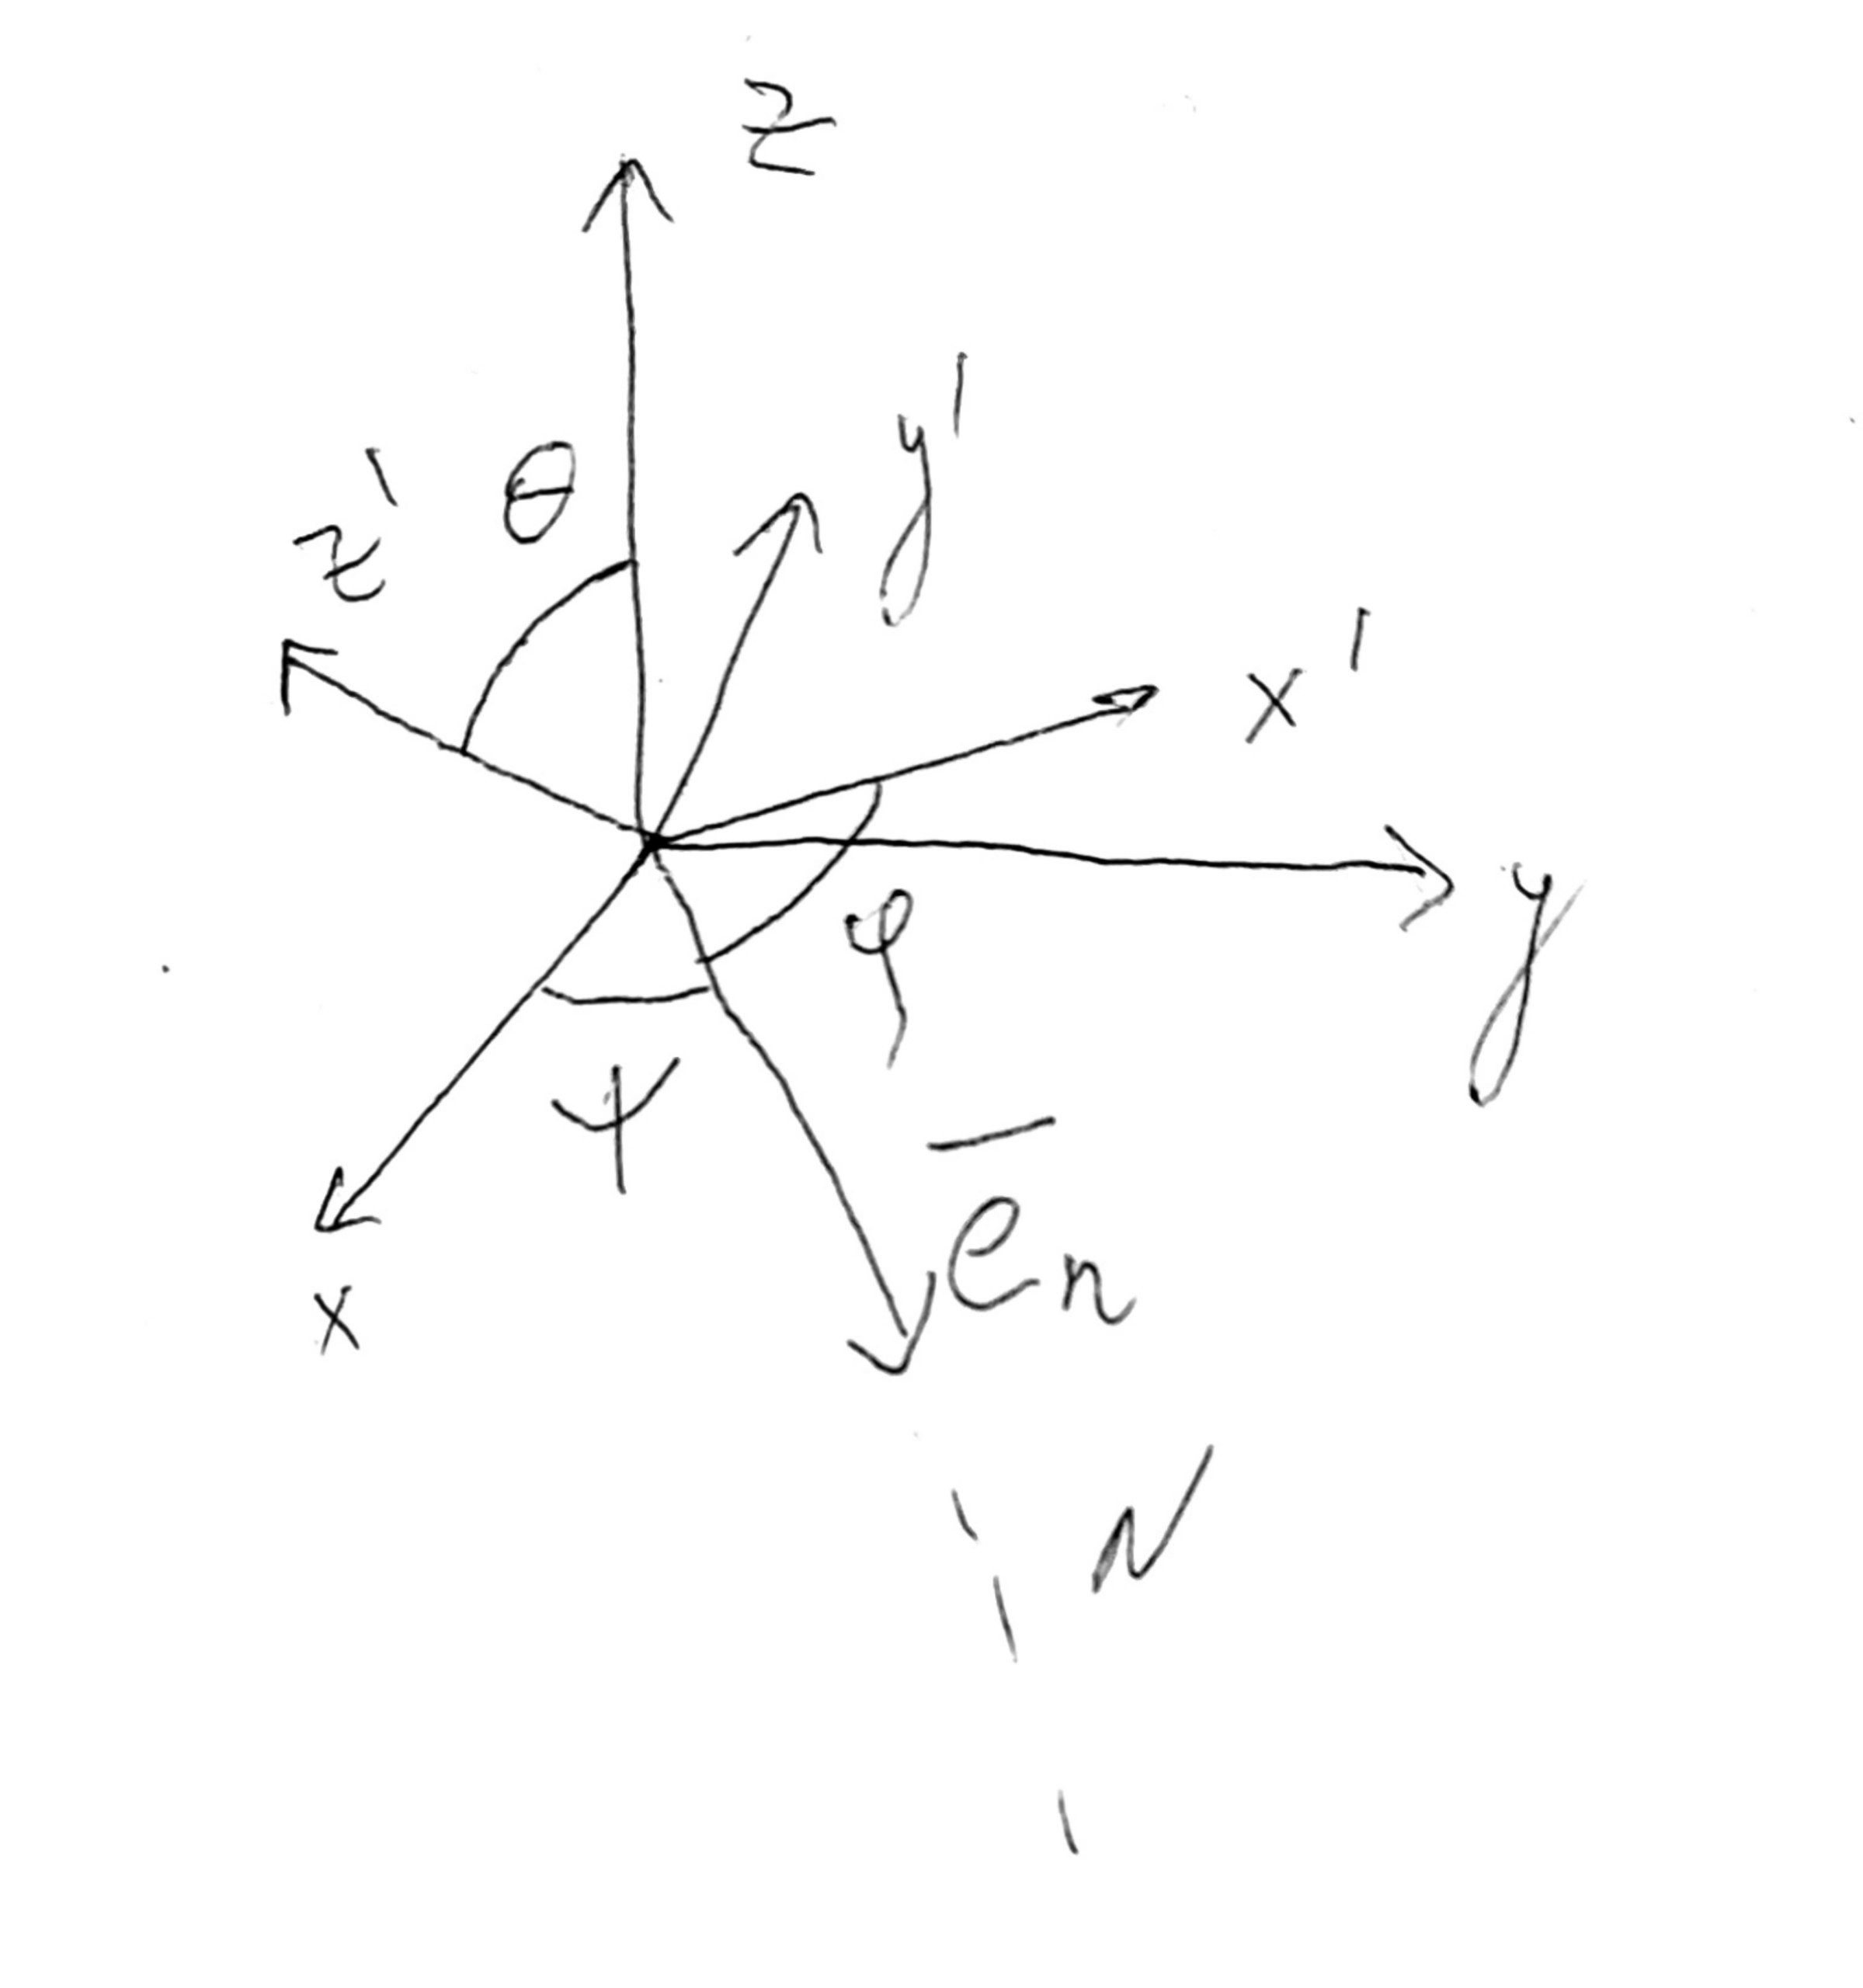
\includegraphics[width=0.5\textwidth]{УглыЭйлера.jpg}
    \caption{}
    \label{fig:myimage} % Sets a label for cross-referencing
\end{figure}
\begin{enumerate}
\item \Def $\theta$ – угол нутации: $\angle (\bar e_z , \bar e_{z'})$
\item $\bar e_n = \frac{\bar e_z \times \bar e_{z'}}{|\bar e_z \times \bar e_{z'}|}$ – Линия узлов
\item $\psi$ – угол прецессии: $\angle (\bar e_x, \bar e_n)$
\item $\varphi$ – угол собственных вращений: $\angle (\bar e_n, \bar e_{x'})$
\end{enumerate}
Замечание: при вращении вокруг оси $z$, углы эйлера вырождаются $\theta =0$

\noindent Замечание: невозможно найти такие 3 числа, чтобы ни при каком случае подобная система не вырождалась

\noindent \keypoint
Теперь можно описать движение тремя функциями(вместо 9 в матрице поворота)
%fixme оформить поровнее, покомпактнее
\[\theta(t) \qquad \psi(t) \qquad \varphi(t) \qquad \qquad \bar \omega = \bar \omega_\theta + \bar \omega_\psi + \bar \omega_\varphi\]
\[\bar \omega_\varphi = \dot {\bar \varphi} \qquad \omega_\theta = \dot {\bar \theta} \qquad \bar \omega_\psi = \dot {\bar \psi}\]
Векторы(которые записаны чуть выше) угловой скорости тогда направлены вдоль осей 
\[\bar \omega_\varphi \| oz' \qquad \bar \omega_\psi \| oz \qquad \bar \omega_\theta \| \bar e_n\]
\[\bar \omega = \begin{pmatrix}
    \omega_x \\ \omega_y \\ \omega_z 
\end{pmatrix}
\qquad
\bar \omega' = 
\begin{pmatrix}
    p \\ q \\ r
\end{pmatrix}
\]
Проецируем на штрихованную систему координат
\[
\begin{array}{l}
    p = (\bar \omega_\theta , \bar e_{x'}) + (\bar \omega_\psi, \bar e_{x'}) + (\bar \omega_\varphi, \bar e_{x'})\\ 
    q = (\bar \omega_\theta, \bar e_{y'}) + (\bar \omega_\psi, \bar e_{y'}) + (\bar \omega_\varphi, \bar e_{y'})\\
    r = (\bar \omega_\theta, \bar e_{z'}) + (\bar \omega_\psi , \bar e_{z'}) + (\bar \omega_\varphi, \bar e_{z'}) 
\end{array}
\implies
%\begin{boxed} %fixme
\begin{cases}
 p = \dot \psi \sin \theta \sin \varphi + \dot \theta \cos \varphi, \\
 q = \dot \psi \sin \theta \cos \varphi - \dot \theta \sin \varphi , \\
 r = \dot \psi \cos \theta + \dot \varphi
\end{cases}
%end{boxed}
\]

\noindent \keypoint 
Уравнения Пуассона для углов Эйлера 
\[
\begin{array}{l}
p\cos \varphi - q \sin \varphi = \dot \theta \left( \cos ^2 \varphi - (- \sin^2 \varphi)\right) \\
p \sin \varphi + q \cos \varphi = \dot \psi (\sin \theta \sin ^2 \varphi + \sin \theta \cos^2\varphi)  \\
\end{array} \implies 
\begin{cases}
    \dot \theta = p \cos \varphi - q \sin \varphi  \\
    \dot \psi = \frac{1}{\sin \theta} \left( p \sin \varphi + q \cos \varphi \right) \\
    \dot \varphi = r - \ctg \theta (p \sin \varphi + q \cos \varphi)
\end{cases}
\]

\noindent \keypoint Упраженение:
\begin{enumerate}
    \item 
    Записать уравнение Пуассона для матрицы направляющих косинусов в пассивной точке зрения
    \item
    Записать уравнения Пуассона для углов Эйлера в активной точке зрения
\end{enumerate}
\section{Кватернионы}
\TwoCols{ %fixme сделать аккуратнее, колхоз с вёрсткой
\[-1 = i^2 = j^2 = k^2 = i \circ j \circ k\]
\[\boxed{q = a + i b + j c + k d}\]
}
{
 %fixme курсив или не курсив
    \centering
    \begin{tabular}{c|c|c|c}
        $1\backslash 2$  & i  & j   & k \\
          \hline
        i & -1 &  k  & -j \\
        \hline
        j & -k & -1  & i \\
        \hline
        k & j &  -i & -1
    \end{tabular}
    \captionof{table}{Таблица перемножения мнимых единиц}
}
\[q = a + \underbracket{i b + j c + k d}_{\bar a} \qquad q= a + \bar a\]
\[
\begin{aligned}
q_1 \circ q_2 &= (a_1 + i b_1 + j c_1 + k d_1) \circ (a_2 + i b_2 + j c_2 + k d_2) \\ 
&= a_1 a_2 + i a_1 b_2 + j a_1 c_2 + k a_1 d_2 + i b_1 a_2 - b_1 b_2 + k b_1 c_2 - j b_1 d_2 + \\
&+ j c_1 a_2 - k c_1 b_2 - c_1 c_2 + i c_1 d_2 + k d_1 a_2 + j d_1 b_2 - i d_1 c_2 - d_1 d_2 \\
&=
a_1 a_2 - b_1 b_2 -c_1 c_2 -d_1 d_2 \\
&+ i \left( a_1 b_2 + b_1 a_2 + c_1 d_2 - d_1 c_2\right) \\
&+ j \left(a_1 c_2 - b_1 d_2 + c_1 a_2 + d_1 b_2\right) \\ 
&+ k \left(a_1 d_2 + b_1 c_2 - c_1 b_2 + d_1 a_2 \right)
\end{aligned}
\]
\[\left( a_1 + \bar a_1\right) \circ \left(a_2 + \bar a_2\right) = a_1 a_2 - (\bar a_1 ,\bar a_2) + a_1 \bar a_2 + a_2 \bar a_1 + \bar a_1 \times \bar a_2 \]
\[a_1 \bar a_2 = i a_1 b_2 + j a_1 c_2 + k a_1 d_2 \]
\[a_2 \bar a_1 = i b_1 a_2 + j c_1 a_2 + k d_1 a_2 \]
\[\bar a_1 \times \bar a_2 = i (c_1 d_2 - d_1 c_2) + j (d_1 b_2 - b_1 d_2) + k (b_1 c_1 - c_1 b_2 )\]
\end{document}
